\documentclass{article}
\usepackage{spconf,amsmath,amssymb,graphicx,booktabs,multirow}
\usepackage{xcolor}
\usepackage{url}
\usepackage{newtxtext,newtxmath}

\title{SetHL: Partially Specified Hand Articulation Control for Video Diffusion}
\name{Haotian Lu \qquad Xiao-Ping Zhang$^{\ast}$}
\address{Tsinghua University\\
haotialu666@gmail.com, xpzhang@ieee.org\thanks{$^{\ast}$Corresponding author.}}

% Automatically generated from locked experiment reports.
\newcommand{\RasterAcc}{56.9}
\newcommand{\RasterAng}{25.13}
\newcommand{\RasterDiv}{12.82}
\newcommand{\RasterAUC}{9.64}
\newcommand{\ContAcc}{51.3}
\newcommand{\ContAng}{30.15}
\newcommand{\ContDiv}{12.12}
\newcommand{\ContAUC}{8.94}
\newcommand{\VQAcc}{51.5}
\newcommand{\VQAng}{29.99}
\newcommand{\VQDiv}{11.36}
\newcommand{\VQAUC}{8.87}
\newcommand{\HardAcc}{52.4}
\newcommand{\HardAng}{29.48}
\newcommand{\HardDiv}{\textbf{12.60}}
\newcommand{\HardAUC}{\textbf{9.15}}
\newcommand{\NoHierAcc}{51.3}
\newcommand{\NoHierAng}{30.63}
\newcommand{\NoHierDiv}{12.42}
\newcommand{\NoHierAUC}{9.10}
\newcommand{\SetAcc}{\textbf{52.9}}
\newcommand{\SetAng}{\textbf{29.04}}
\newcommand{\SetDiv}{11.71}
\newcommand{\SetAUC}{8.59}
\newcommand{\PrimaryDelta}{-0.35}
\newcommand{\PrimaryCI}{[-1.06, 0.34]}
\newcommand{\VQDelta}{-0.29}
\newcommand{\VQCI}{[-0.80, 0.18]}
\newcommand{\SphericalDelta}{-0.52}
\newcommand{\SphericalCI}{[-0.88, -0.14]}
\newcommand{\HardDelta}{-0.57}
\newcommand{\HardCI}{[-1.089, -0.005]}
\newcommand{\CenterAUC}{8.86}
\newcommand{\CenterDelta}{-0.27}
\newcommand{\CenterCI}{[-0.62, 0.11]}
\newcommand{\ContAccDelta}{1.59}
\newcommand{\ContAccCI}{[0.47, 2.79]}
\newcommand{\ContAngDelta}{-1.11}
\newcommand{\ContAngCI}{[-2.33, -0.04]}
\newcommand{\ContLeakDelta}{-3.87}
\newcommand{\ContLeakCI}{[-6.05, -1.72]}
\newcommand{\ContDetectionDelta}{3.47}
\newcommand{\ContDetectionCI}{[1.94, 5.06]}
\newcommand{\ContLocalizedDelta}{-0.41}
\newcommand{\ContLocalizedCI}{[-1.80, 1.04]}
\newcommand{\VQAccDelta}{1.34}
\newcommand{\VQAccCI}{[0.12, 2.63]}
\newcommand{\VQLeakDelta}{-2.80}
\newcommand{\VQLeakCI}{[-4.97, -0.77]}
\newcommand{\SphericalAccDelta}{1.56}
\newcommand{\SphericalAccCI}{[0.51, 2.65]}
\newcommand{\SphericalAngDelta}{-1.59}
\newcommand{\SphericalAngCI}{[-3.07, -0.43]}
\newcommand{\CompSetAng}{24.47}
\newcommand{\CompContAng}{17.96}
\newcommand{\CompSetAcc}{54.7}
\newcommand{\CompContAcc}{61.8}
\newcommand{\CompSphericalGain}{0.57}
\newcommand{\HLQuantDeg}{16.91$^\circ$}
\newcommand{\VQQuantDeg}{16.16$^\circ$}
\newcommand{\HLStability}{46.3\%}
\newcommand{\VQStability}{45.6\%}
\newcommand{\PosteriorTemperature}{1}
\newcommand{\DenoiseSet}{0.1023}
\newcommand{\DenoiseCont}{0.1053}
\newcommand{\DenoiseDelta}{-0.0030}
\newcommand{\DenoiseCI}{[-0.0035, -0.0024]}
\newcommand{\DenoiseRelative}{2.81}
\newcommand{\ResultSentence}{SetHL obtains 8.59 hypervolume, versus 8.94 for continuous and 8.87 for VQ-26.}
\newcommand{\FullControlSentence}{Under full articulation control, SetHL obtains 52.9\% HL accuracy versus 51.3\% for continuous control (paired difference 1.64 points, 95\% CI [0.42, 2.98]).}


\begin{document}
\maketitle

\begin{abstract}
Pose-conditioned video generators assume complete trajectories, although users
may specify only semantically important fingers or intervals. We formulate
\emph{partially specified hand control}: obey declared constraints while
preserving variation elsewhere. SetHL extends Hand Labanotation (HL) from fixed
symbols to distributions over unspecified cells. A masked transformer completes
missing symbols, a certified in-cell sampler supplies continuous variation
without changing HL labels, and a kinematic layer drives a
Wan2.1-Fun-Control 1.3B model trained with rank-16 LoRA. On quality-filtered
WLASL, matched three-seed experiments show that SetHL improves specified-symbol
accuracy over continuous and learned vector-quantized controls by 1.59 and 1.34
points, and reduces leakage by 3.87 and 2.80 points. The primary
compliance--diversity hypervolume differences are not significant, while
conditional denoising MSE improves by \DenoiseRelative\% versus continuous
control. These results support structured partial constraints as an editable
interface for video diffusion while separating controlled from free hand
articulation.
\end{abstract}

\begin{keywords}
controllable video generation, hand motion, Hand Labanotation, diffusion models
\end{keywords}

\section{Introduction}
\label{sec:intro}
Hand motion is both semantically dense and difficult to synthesize.  Many
pose-based controllers consume a complete joint trajectory, while sparse-control
methods usually sparsify time or landmarks rather than letting authors declare
which articulations are unconstrained~\cite{controlnet,sparsectrl,motioni2v,motionctrl}.
Complete trajectories are suitable for reenactment, but form a poor
authoring interface: a user may require an index finger to point inward during
one interval while leaving the remaining articulation unspecified.  Treating
missing coordinates as zeros or hallucinating a single completed skeleton
confuses ``free to vary'' with ``fixed to an arbitrary estimate.''

Hand Labanotation (HL)~\cite{li2024hl} provides a useful alternative.  It
describes each of 20 hand-local bone directions by one of 26 interpretable
spatial symbols.  The original work used HL for recognition, documentation,
and approximate one-shot skeleton recovery.  We ask a different question:
can a partial symbolic program define a \emph{set} of valid videos rather than
one trajectory?

We propose SetHL-Wan.  Specified HL symbols are transmitted exactly, whereas a
temporal completion network represents each unspecified cell by a categorical
posterior.  Samples are forward-kinematically spatialized and lifted to the
control-latent interface of Wan~\cite{wan}.  Only low-rank adapters~\cite{lora}, the
completion network, and the lifting module are trained.  Crucially, no dense
joint coordinates bypass the symbolic stream.

Our contributions are: (1) a task definition and metric that jointly measures
constraint compliance and diversity localized to unconstrained hand parts;
(2) a probabilistic extension of HL with certified symbol-preserving continuous
samples, coupled to a differentiable kinematic Wan controller; and (3)
matched-budget tests against continuous and learned-token
alternatives, including structured missing-control and noise stress tests.

\begin{figure*}[t]
\centering
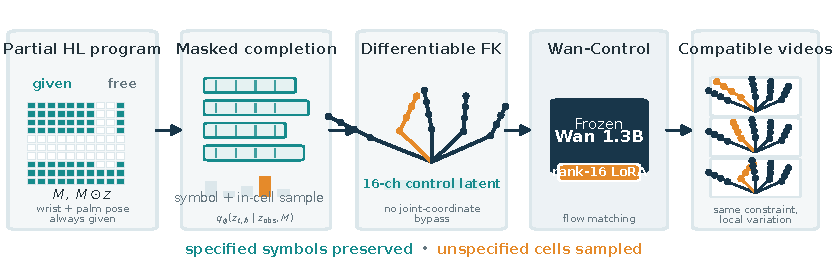
\includegraphics[width=\textwidth]{figures/method_overview.pdf}
\caption{SetHL treats a partial hand instruction as a set rather than a single
completed skeleton. Given HL cells are copied exactly; a masked transformer
predicts distributions for free cells, which are sampled and spatialized by
forward kinematics before conditioning a LoRA-adapted Wan model. Continuous
within-cell samples preserve their selected HL symbol by construction.}
\label{fig:method}
\end{figure*}

\section{Related Work}
\label{sec:related}
\textbf{Controllable video diffusion.}
ControlNet~\cite{controlnet} established spatial conditioning for diffusion
models, while SparseCtrl~\cite{sparsectrl} studied temporally sparse video
conditions. Recent work conditions video models on pose or trajectories
~\cite{motioni2v,motionctrl,posetraj,wanmove,motionprompt}. Sparse 3-D hand control has
also addressed occlusion and geometric fidelity~\cite{sparse3dhand}, but
``sparse'' there describes landmarks or missing observations, not
author-declared degrees of freedom. These methods seek one accurate motion
trace; our target is selective constraint with localized residual variation.
Learned 3-D motion and mesh tokens avoid rasterized controls
~\cite{mtvcraft,meshtoken}, but encode complete motion with task-specific
vocabularies rather than an interpretable, partially specified program.

\textbf{Hand and sign generation.}
WLASL~\cite{wlasl} enables large-scale word-level sign recognition.  Recent
generators improve sign fidelity through pose adapters~\cite{signrefine} or
compressed multimodal tokens~\cite{signvip}.  They motivate stronger hand
evaluation, but do not expose a symbolic partial-control interface.

\textbf{Symbolic hand motion.}
HL~\cite{li2024hl} quantizes hand-local directions and is robust to small pose
noise.  We retain its fixed semantics, but replace deterministic cell-center
recovery with a posterior over unspecified cells and train it as a generative
condition.  A learned 26-entry VQ codebook is included to test whether gains
come merely from discretization.

\section{Method}
\label{sec:method}
Let $X=(x_1,\ldots,x_T)$ be a video and $J_t\in\mathbb{R}^{2\times21\times3}$
its two-hand landmarks.  The control mask $M\in\{0,1\}^{T\times2\times20}$
indicates which bone-time cells the user specifies.

\subsection{Partial Hand-Labanotation programs}
For each hand we construct the palm frame $R_t$ from the wrist, index
metacarpophalangeal joint, middle metacarpophalangeal joint, and little-finger
metacarpophalangeal joint as in~\cite{li2024hl}.  A bone direction $d_{t,b}$ is
mapped into this frame and assigned to its nearest member of the fixed
26-direction codebook $C=\{c_k\}_{k=1}^{26}$:
\begin{equation}
 z_{t,b}=\arg\max_k\langle R_t^\top d_{t,b},c_k\rangle .
\end{equation}
The transmitted program contains $(M,M\odot z)$, wrist trajectories, palm
frames, and reference bone lengths.  It never contains per-joint image
coordinates. Specified cells are one-hot, preventing continuous sub-cell
information from leaking through soft labels. We interpret each symbol as its
spherical Voronoi cell rather than only its center.

For missing cells, a transformer $q_\phi$ attends jointly over time, hands,
and the 20-bone trees:
\begin{equation}
\begin{aligned}
 q_{t,b}&=q_\phi(z_{\mathrm{obs}},M),\\
 \mathcal L_{\mathrm{HL}}&=-\log q_{t,b}(z_{t,b})
 +\lambda_h[1-\langle\bar c_{t,b},c_{z_{t,b}}\rangle].
\end{aligned}
\end{equation}
where $\bar c$ is the normalized posterior mean.  The second term respects
the geometry of nearby HL regions instead of treating all symbol mistakes as
equally severe.

\subsection{Kinematic control-latent lifting}
A hard straight-through categorical sample first selects a center $c_z$. For
unit $v\perp c_z$, we draw
\begin{equation}
 \tilde d=\cos\alpha\,c_z+\sin\alpha\,v,\quad
 \alpha<\tfrac12\min_{j\ne z}\arccos(c_z^\top c_j).
\end{equation}
By the spherical triangle inequality, $c_z$ remains the nearest codeword. This
gives continuous variation with a certificate that the HL instruction is
unchanged. Forward
kinematics reconstructs bone endpoints from wrist position, palm frame, and
bone length. Bone tokens are bilinearly splatted along their 2-D
segments and decoded by three small 3-D convolutions into a 16-channel latent
$H_\psi(P)$ at Wan's temporal and spatial resolution.  We concatenate it with
the first-frame latent, matching the native Wan-Control input contract.

Given clean latent $v$, noise $\epsilon$, and flow-matching interpolation
$v_\sigma=(1-\sigma)v+\sigma\epsilon$, we optimize
\begin{equation}
 \mathcal L=\|f_{\theta,\Delta}(v_\sigma,\sigma,H_\psi(P))
 -(\epsilon-v)\|_2^2+0.1\mathcal L_{\mathrm{HL}},
\end{equation}
where the 1.3B Wan backbone $\theta$ is frozen and $\Delta$ denotes rank-16
LoRA parameters. At inference, independent posterior samples alter the
control trajectory only where the program permits it, while diffusion noise
supplies appearance variation.

\begin{figure*}[t]
\centering
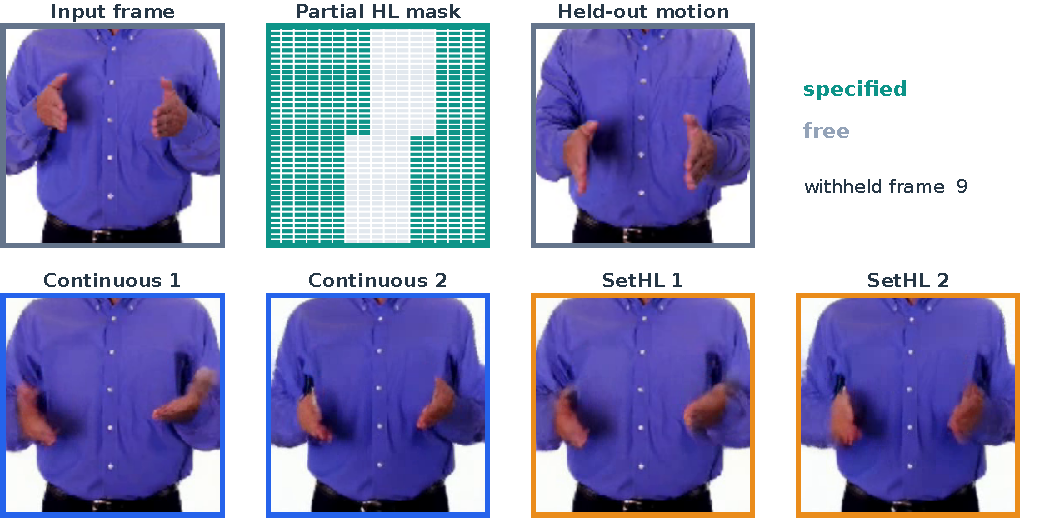
\includegraphics[width=\textwidth]{figures/qualitative.pdf}
\caption{Generated-video comparison on the source at the median three-seed
SetHL hypervolume (a deterministic selection rule). Teal mask cells are
specified and gray cells are free; frames are taken at the center of the
withheld interval. Columns show paired diffusion seeds under continuous and
SetHL control.}
\label{fig:qualitative}
\end{figure*}

\section{Experiments}
\label{sec:experiments}
\textbf{Data and protocol.}
We use 2,252 WLASL videos with reliable MediaPipe Hands~\cite{mediapipe}
tracks, retaining the official 1,579/404/269 train/validation/test partition.
Each source video contributes exactly one 17-frame clip; no overlapping window
crosses a split. Frames are resized to $256^2$. Every learned method uses
the same Wan checkpoint, rank-16 LoRA, 3,000 updates, and three seeds.
SetHL trains 21.85M parameters in total (LoRA plus its completion and lifting
modules), while the matched continuous model trains 21.84M.
With cached Wan-VAE latents, each 3,000-step seed takes about 28 minutes on one
Ascend 910B2C NPU.
Text and CLIP embeddings are fixed to zero for every method so the comparison
isolates first-frame and motion-control conditioning.
We select $\lambda_h=1$ from $\{0,0.25,1\}$ using validation data only.
We likewise select posterior temperature \PosteriorTemperature{} from
$\{1,1.5,2\}$ on eight fixed validation sources and share it across all
probabilistic categorical controls.

\textbf{Baselines and metrics.}
We compare continuous Gaussian directions, a training-set 26-entry VQ
codebook, hard HL centers, SetHL without the spherical loss, and full SetHL.
Continuous and raster controls retain exact observed geometry and therefore
serve as information-richer upper bounds, while parameter counts and training
updates remain matched.
At inference we also disable within-cell residuals in the trained SetHL model,
isolating their contribution without changing learned weights.
Training samples masks that remove a distal joint set, one complete finger, or
a contiguous temporal interval.  Standalone completion averages all three;
the primary generated-video benchmark uses the predeclared interval mask. A
secondary robustness policy is selected between finger and distal masks on the
fixed eight-source validation subset, then evaluated once on the test set. We report specified-symbol accuracy, specified angular error,
hidden-cell angular diversity, specified-cell symbol disagreement, hand
detection, temporal acceleration error, and denoising MSE. The primary endpoint
is the Pareto hypervolume dominated by compliance--localized-diversity operating
points (reference $(0,0)$) obtained by scaling the control latent. Localized
diversity multiplies hidden-cell angular diversity by semantic agreement on
specified cells and hand-detection rate. Thus semantic leakage and untrackable
hands are penalized while legal angular variation inside an HL cell is not.
Confidence intervals use 10,000 paired bootstrap resamples of source videos.
Generated-video metrics use all 27 test clips meeting the fixed criterion
that both hands are tracked in at least 90\% of source frames.
As an evaluator ceiling, re-encoding these real clips and rerunning the same
tracker gives 92.81\% hand detection, 78.36\% HL agreement, and
$10.24^\circ$ angular error against the archived pseudo-labels.
As a post-hoc quality diagnostic, we also measure source-conditioned cosine
similarity in the penultimate feature space of a Kinetics-400-pretrained
R3D-18~\cite{r3d}; this metric was not used for model selection.

\begin{table}[t]
\caption{Interval partial-control results on the WLASL test split. Higher is better for
accuracy, localized diversity, and hypervolume; lower is better for angle. Values average
three training seeds; bold marks the best 26-symbol method, and paired 95\%
intervals are reported in text.}
\label{tab:main}
\centering
\small
\setlength{\tabcolsep}{2.8pt}
\begin{tabular}{lcccc}
\toprule
Method & Acc.(\%)$\uparrow$ & Ang.$^\circ\downarrow$ & LocDiv$^\circ\uparrow$ & HV$\uparrow$\\
\midrule
\multicolumn{5}{l}{\emph{Information-rich controls}}\\
Raster skeleton & \RasterAcc & \RasterAng & \RasterDiv & \RasterAUC\\
Continuous Gauss. & \ContAcc & \ContAng & \ContDiv & \ContAUC\\
\midrule
\multicolumn{5}{l}{\emph{26-symbol controls}}\\
Learned VQ-26 & \VQAcc & \VQAng & \VQDiv & \VQAUC\\
Hard HL & \HardAcc & \HardAng & \HardDiv & \HardAUC\\
SetHL w/o sph. loss & \NoHierAcc & \NoHierAng & \NoHierDiv & \NoHierAUC\\
SetHL-Wan & \SetAcc & \SetAng & \SetDiv & \SetAUC\\
\bottomrule
\end{tabular}
\end{table}

\textbf{Main results.}
Table~\ref{tab:main} reports the locked comparison.  \ResultSentence{}
The paired SetHL--continuous difference in the primary endpoint is
\PrimaryDelta{} (95\% CI \PrimaryCI); against VQ-26 it is
\VQDelta{} (\VQCI). The predeclared HV-superiority criterion is therefore not
met; SetHL nevertheless has the best accuracy and angular error among the
matched 26-symbol controllers. Against the no-spherical-loss ablation, SetHL
changes accuracy by \SphericalAccDelta{} points (\SphericalAccCI), angle by
\SphericalAngDelta$^\circ$ (\SphericalAngCI), and HV by \SphericalDelta{}
(\SphericalCI). Center-only and hard-HL inference reach \CenterAUC{} and
\HardAUC{} HV, respectively, confirming that spherical geometry favors
semantic compliance rather than uniformly increasing diversity.
Relative to continuous control, SetHL changes specified accuracy by
\ContAccDelta{} percentage points (\ContAccCI), angular error by \ContAngDelta$^\circ$
(\ContAngCI), leakage by \ContLeakDelta{} points (\ContLeakCI), and detection
by \ContDetectionDelta{} points (\ContDetectionCI); its localized-diversity
difference is \ContLocalizedDelta$^\circ$ (\ContLocalizedCI).
Against learned VQ-26, SetHL changes specified accuracy by \VQAccDelta{} percentage points
(\VQAccCI) and leakage by \VQLeakDelta{} points (\VQLeakCI).
A validation-selected whole-finger mask reproduces the semantic advantage over
continuous control: accuracy changes by \FingerAccDelta{} points (\FingerAccCI),
angle by \FingerAngDelta$^\circ$ (\FingerAngCI), leakage by
\FingerLeakDelta{} points (\FingerLeakCI), detection by
\FingerDetectionDelta{} points (\FingerDetectionCI), and acceleration error by
\FingerAccelDelta{} (\FingerAccelCI). Its HV change is \FingerHVDelta{}
(\FingerHVCI), so frontier superiority remains unsupported.
\FullControlSentence{} On all 269 test clips, interval-conditioned denoising
MSE is \DenoiseSet{} for SetHL and \DenoiseCont{} for continuous control
(paired change \DenoiseDelta{}, 95\% CI \DenoiseCI).
R3D feature similarity is \VideoFeatureSet{} versus \VideoFeatureCont{}
(paired change \VideoFeatureDelta{}, 95\% CI \VideoFeatureCI), indicating no
loss of source-level video consistency alongside the semantic gains.

\textbf{Representation analysis.}
On held-out directions, fixed HL has \HLQuantDeg{} mean quantization error,
versus \VQQuantDeg{} for VQ-26.  Under coordinate noise $\sigma=0.005$, however,
HL retains \HLStability{} of symbols compared with \VQStability{} for VQ.
This separates geometric precision from stability and tests whether a learned
vocabulary alone explains the result. Standalone masked completion favors the
continuous model (\CompContAng$^\circ$/\CompContAcc\%) over SetHL
(\CompSetAng$^\circ$/\CompSetAcc\%); the spherical term nevertheless reduces
SetHL completion error by \CompSphericalGain$^\circ$. Thus the video comparison
does not conflate set-valued control with nearest-trajectory imputation.

\section{Conclusion}
Partial hand instructions should define constraints, not prematurely collapse
generation to one completed skeleton.  SetHL extends a fixed, interpretable
notation into a distribution-valued controller for Wan.  Its value is tested
by where variation occurs, not merely by whether generated motion is diverse.
The present evaluation is limited to short, hand-focused WLASL clips and
tracker-derived pseudo-labels; broader domains and human judgments remain
future work.

\section{Compliance with Ethical Standards}
This study used only the publicly available WLASL dataset and involved no new
data collection or interaction with human participants; no ethical approval
was required.

\section{Acknowledgment}
OpenAI Codex assisted with language drafting throughout the manuscript,
implementation of evaluation and statistical-analysis code, and scripting of
Figs.~1--2. The authors reviewed all outputs and take responsibility for the
study design, paper content, and reported results.

\bibliographystyle{IEEEbib}
\bibliography{refs}
\end{document}
